\subsection{Trilateration}

\subsubsection*{Rechnerische Lösung}

Um die Position rechnerisch zu bestimmen, habe ich zunächst für jeden der vier Access Points (im Folgenden APs genannt) die entsprechende Gleichung aufgestellt. Die Formel aus der Angabe lautet:

\begin{equation*}
    |r_n| = \sqrt{(x_n - x)^2 + (y_n - y)^2}
\end{equation*}
und kann leicht zu folgender Gleichung vereinfacht werden:
\begin{equation*}
    |r_n|^2 = (x_n - x)^2 + (y_n - y)^2
\end{equation*}
Die Gleichungen lauten dann:


\begin{subequations}
    \begin{empheq}{align}
        158.76  &=  x^2 + y^2\label{eq:1}\\
        116.64  &=  (20-x)^2 + y^2\\
        475.24  &=  (5-x)^2 + (15-y)^2\\
        368.64  &=  (18-x)^2 + (12-y)^2
    \end{empheq}
\end{subequations}

Als nächstes können die Quadrate aufgelöst, also ausmultipliziert, werden.

\begin{subequations}
    \begin{empheq}{align}
        \stepcounter{equation}
        116.64  &=  400 - 40x + x^2 + y^2\\
        475.24  &=  25 - 10x + x^2 + 225 - 30y + y^2\\
        368.64  &=  324 - 36x + x^2 + 144 - 24y + y^2
    \end{empheq}
\end{subequations}


\begin{subequations}
    \begin{empheq}{align}
        \stepcounter{equation}
        \stepcounter{equation}
        475.24  &=  250 - 10x + x^2 - 30y + y^2\\
        368.64  &=  468 - 36x + x^2 - 24y + y^2
    \end{empheq}
\end{subequations}

\begin{subequations}
    \begin{empheq}{align}
        \stepcounter{equation}
        116.64 - 400 &=  - 40x + x^2 + y^2\\
        475.24 - 250 &=  - 10x + x^2 - 30y + y^2\\
        368.64 - 468 &=  - 36x + x^2 - 24y + y^2
    \end{empheq}
\end{subequations}

\begin{subequations}
    \begin{empheq}{align}
        \stepcounter{equation}
        -283.36 &=  - 40x + x^2 + y^2\label{eq:2}\\
        225.24 &=  - 10x + x^2 - 30y + y^2\label{eq:3}\\
        -99.36 &=  - 36x + x^2 - 24y + y^2\label{eq:4}
    \end{empheq}
\end{subequations}
Die Gleichung \ref{eq:1} kann nun nach $y^2$ umgestellt werden:
\begin{equation*}
    y^2 = 158.76 - x^2
\end{equation*}
und danach in die Gleichung \ref{eq:2} eingesetzt werden:
\begin{align*}
    -283.36 & =  - 40x + x^2 + 158.76 - x^2 \\
    -283.36 & =  - 40x + 158.76             \\
    -442.12 & =  - 40x                      \\
    x       & = 11.053
\end{align*}
Nun kann $x$ in die Gleichung \ref{eq:3} eingesetzt werden:
\begin{align*}
    225.24                     & =  - 10 \cdot 11.053 + 11.053^2 - 30y + y^2 \\
    225.24 + 110.53 - 11.053^2 & = -30y + y^2                                \\
    0                          & = y^2 - 30y - 214.601191
\end{align*}
Diese quadratische Gleichung kann nun mit der Mitternachtsformel gelöst werden, was die beiden Lösungen $y_1 = -5.94281$ und $y_2 = 35.9428$ ergibt.

Wenn man nun erst $x$ in die Gleichung \ref{eq:4} einsetzt, ergibt sich:
\begin{align*}
    -99.36                      & = -36x + x^2 - 24y + y^2                  \\
    -99.36                      & = -36 \cdot 11.053 + 11.053^2 - 24y + y^2 \\
    -99.36 + 397.908 - 122.1688 & =  - 24y + y^2                            \\
    0                           & = y^2 - 24y - 176.3792
\end{align*}
Wenn man dann noch die beiden möglichen Werte für $y$ einsetzt, ergeben sich folgende Gleichungen:
\begin{align*}
    0 & = (-5.94281)^2 - 24 \cdot (-5.94281) - 176.3792
      & = 1.56523                                                    \\
    0 & = (35.9428)^2 - 24 \cdot (35.9428) - 176.3792   & = 252.8784
\end{align*}

Dies ist ein offensichtlicher Widerspruch, der darauf hinweist, dass es keine exakte Lösung gibt, sich das Objekt X aber in der Nähe der Koordinaten $(11, -6)$ befinden muss.

Als Test können wir zusätzlich die vorletzte Gleichung lösen:
\begin{align*}
    0 & = y^2 - 24y - 176.3792
\end{align*}
was die Lösungen $y_1 = -5.89914$ und $y_2 = 29.8991$ ergibt.

Die y-Werte $35.9428$ und $29.8991$ können ausgeschlossen werden, da
\begin{align*}
    29.8991^2 + 11.053^2 & = 1016.12498 \gg 116.64 \\
    35.9428^2 + 11.053^2 & = 1414.0536 \gg 116.64
\end{align*}
mit der Gleichung \ref{eq:1} deutlich weniger übereinstimmt als die niedrigeren Werte.
\begin{align*}
    -5.89914^2 + 11.053^2 & = 156.9686 \approx 116.64 \\
    -5.94281^2 + 11.053^2 & = 157.4857 \approx 116.64
\end{align*}


\subsubsection*{Graphische Validierung}

Die errechnete Lösung kann zudem recht leicht graphisch verifiziert werden. Dazu werden zuerst die Punkte, die die Standorte der APs darstellen geplottet (hier in GeoGebra). Anschließend werden die 4 Gleichungen hinzugefügt. Wie zu erwarten, entsteht dadurch für jeden AP ein Kreis mit diesem AP als Mittelpunkt, die Durchmesser sind aber jeweils verschieden.

Auch wenn es auf den ersten Blick so aussieht, als ob es eine exakte Lösung gäbe: Spätestens beim Heranzoomen wird klar, dass sich an keinem einzigen Punkt auch nur drei der vier Kreise schneiden.

\begin{figure}[H]
    \centering
    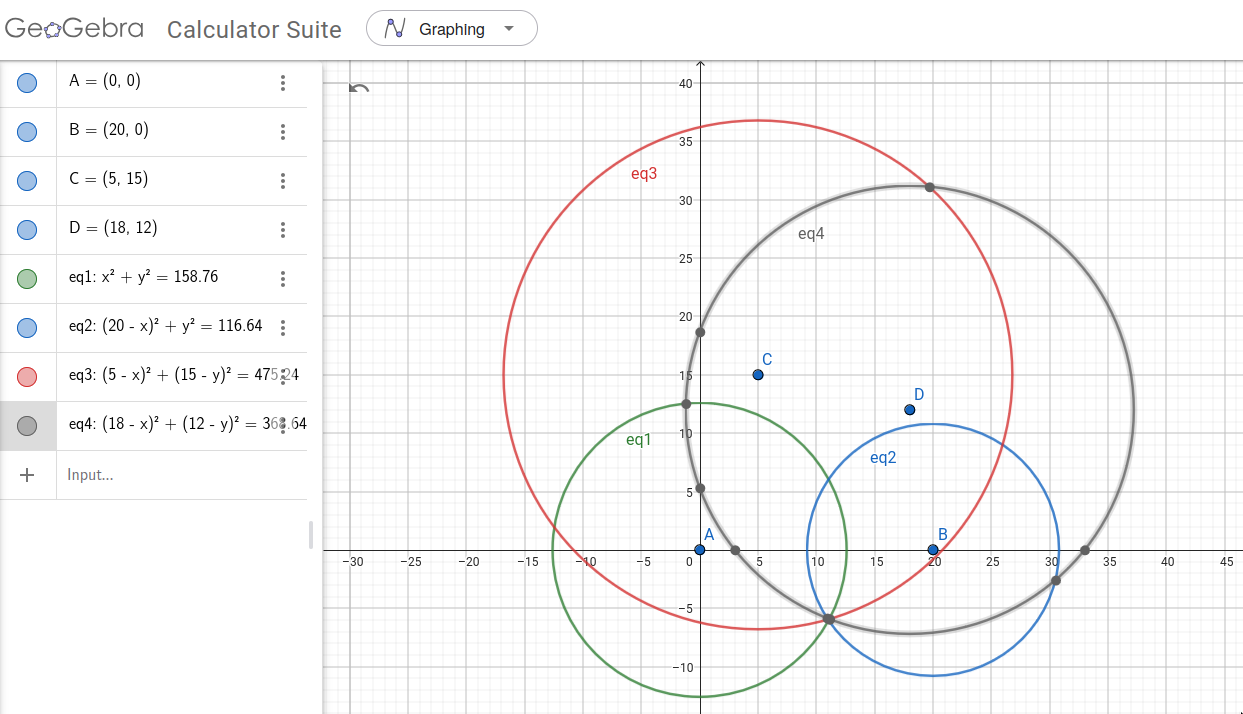
\includegraphics[width=0.5\textwidth]{figures/geogebra/screen_2.png}
    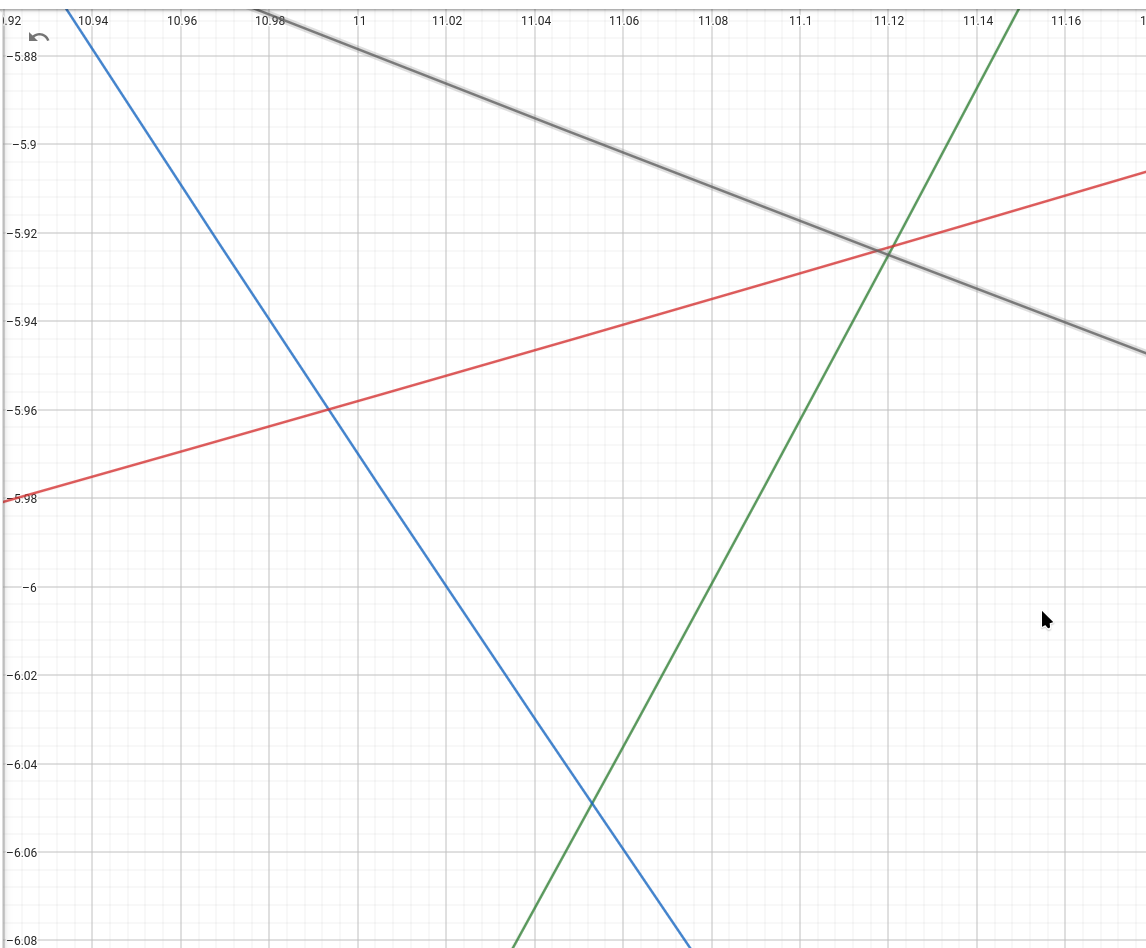
\includegraphics[width=0.4\textwidth]{figures/geogebra/screen_3.png}
    \caption{Graphische Validierung der errechneten Lösung mit GeoGebra. Links sind die konzentrischen Kreise um die vier APs zu sehen, rechts der vermeintliche Schnittpunkt der Kreise.}
    \label{geogebra}
\end{figure}

\subsubsection*{Ergebnis}

Es kann also kein exaktes Ergebnis bestimmt werden, was auch nicht überraschend ist, da die Messwerte ja Ungenauigkeiten unterliegen.
Das Objekt X befindet sich also in der Nähe der, aber nicht exakt an den, Koordinaten $(11, -6)$, was auch durch die graphische Validierung bestätigt wird.